\clearpage
\subsection{premi/client/trailMap}
\begin{figure}[H]
\begin{center}
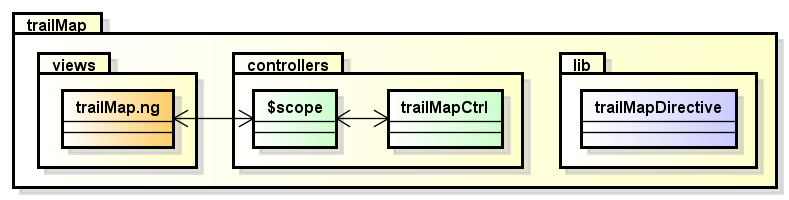
\includegraphics[scale=0.70]{img/diapkg/trailMap.png}
\caption{Diagramma della classe premi/client/trailMap}
\end{center}
\end{figure}

%-------  diagramma di un template %
\subsubsection{premi/client/trailMap/views/trailMap.ng}

\begin{description}
%-------  descrizione del template%
\item[Descrizione] \hfill
	Template della vista associata allo \textit{\$scope} di \textit{trailMapCtrl} che visualizza una mappa per un determinato trail. Nella sezione Frames Out sono presenti i frame che non sono presenti nel trail e che possono essere aggiunti. Nella sezione Trail è presente un menù che permette di aggiungere un checkpoint e di aggiungere i frame nel trail. 
\end{description}

%-------  diagramma della classe%
\subsubsection{premi/client/trailMap/controllers/trailMapCtrl}
\begin{figure}[H]
\begin{center}
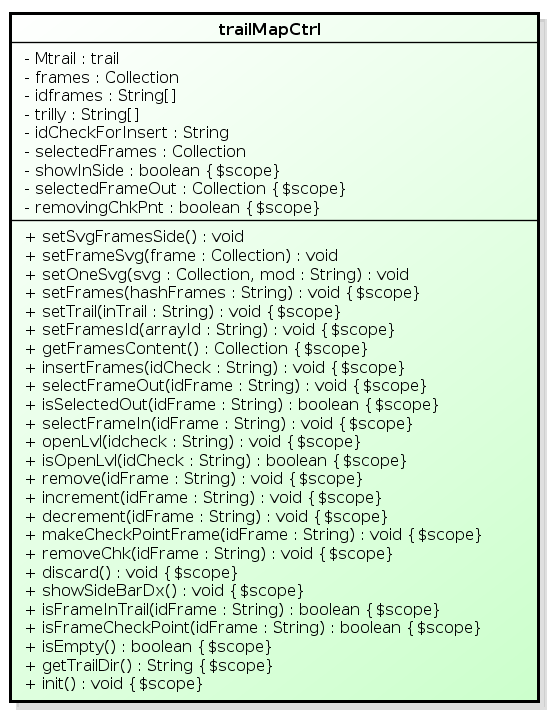
\includegraphics[scale=0.85]{img/diacla/TrailMapCtrl.png}
\caption{Diagramma della classe premi/editor/controllers/trailMapCtrl}
\end{center}
\end{figure}


\begin{description}
%-------  descrizione della classe%
\item[Descrizione] \hfill
	Controller della view \textit{trailMap.ng}. Fornisce, tramite lo \textit{\$scope} i metodi per la modifica o l'aggiunta delle slide che formano il percorso di un trail. 
	\\ La dicitura \{\$scope\} nel diagramma UML$_G$ indica che:
\begin{itemize}
\item tutti gli attributi e i metodi pubblici del controller vanno inseriti nello \$scope;
\item tutti gli attributi e i metodi privati del controller appartengono al controller.
\end{itemize}
Vedere la sezione \ref{servizi} per approfondimenti sull'oggetto \$scope.
	
%-------  lista degli Attributi%	
\item[Attributi] \hfill
	\begin{description}
		\item[\textbf{- Mtrail : trail			}] \hfill
			Oggetto Trail da modificare. Inizialmente vuoto, dev’essere inizializzato
con gli attributi di trailCollection
		\item[\textbf{- frames : collection			}] \hfill
			contiene	 degli oggetti JSON che rappresentano i frames appartenenti al trail che si sta modificando
		\item[\textbf{- idframes : Array			}] \hfill			
			array che contiene gli identificativi dei frames appartenenti al trail che si sta modificando		
		\item[\textbf{- trilly : Array			}] \hfill			
			Matrice vuota, utilizzata come variabile d’appoggio per l’utilizzo del metodo
di MTrail initPath per la sua inizializzazione
		\item[\textbf{- selectedFrames : collection			}] \hfill			
			contiene gli oggetti JSON dei frames che sono stati selezionati nella vista trailMap.ng
		\item[\textbf{+ showInSide : boolean			}] \hfill			
			Indica se la barra di destra dell’editor dev’essere visualizzata (true) o meno
(false)
		\item[\textbf{+ selectedFrameOut : collection			}] \hfill			
			contiene gli oggetti JSON dei frames che sono stati selezionati nella vista trailMap.ng nella sezione Frames Out
		\item[\textbf{+ removingChkPnt : boolean			}] \hfill			
			se settata a true consente a removeChk di togliere un checkpoint, se settata a false l'operazione viene annullata	
		\item[\textbf{+ selectedLvls : array			}] \hfill			
			contiene i riferimenti dei Frame che sono checkpoint	
	\end{description}
	
	
%-------  lista dei metodi%	
\item[Metodi] \hfill

	% -- inizio metodo -- %
	\begin{description}
		\item[\textbf{\color{blue}- setOneSvg(svg : collection, mod : String) : void			}] \hfill
		tramite due metodi JQuery$_G$ setta il colore e il path dell'svg.		
			
		\begin{description}
			% -- lista argomenti del metodo -- %
			\item[Argomenti] \hfill
				\begin{itemize}
				
					\item \textbf{svg : collection			} \hfill
						un oggetto JSON che identifica un svg
					\item \textbf{mod : String			} \hfill
						identifica gli id HTML$_G$ associati all'svg
				\end{itemize}
		\end{description}
	\end{description}
	% -- fine metodo -- %

% -- inizio metodo -- %
	\begin{description}
		\item[\textbf{\color{blue}- setFrameSvg(frame : collection) : void			}] \hfill
			chiama il metodo setOneSvg per ogni shape contenuto nel frame ricevuto in input	
			
		\begin{description}
			% -- lista argomenti del metodo -- %
			\item[Argomenti] \hfill
				\begin{itemize}
				
					\item \textbf{frame : collection			} \hfill
						un oggetto JSON che rappresenta un frame
				\end{itemize}
		\end{description}
	\end{description}
	% -- fine metodo -- %
	
	% -- inizio metodo -- %
	\begin{description}
		\item[\textbf{\color{blue}- setSvgFramesSide() : void			}] \hfill
			per ogni frame appartenente al trail viene chiamato il metodo setFrameSvg	
			
	\end{description}
	% -- fine metodo -- %
	
	
	% -- inizio metodo -- %
	\begin{description}
		\item[\textbf{\color{blue}+ setFrames(hashFrames : list) : void			}] \hfill
			inserisce i frame nella lista dei frames convertendo la lista in input in oggetti JSON di tipo frame
			
		\begin{description}
			% -- lista argomenti del metodo -- %
			\item[Argomenti] \hfill
				\begin{itemize}
				
					\item \textbf{hashFrames : list			} \hfill
						lista di frame da convertire
					
				\end{itemize}
		\end{description}
	\end{description}
	% -- fine metodo -- %	
	
		% -- inizio metodo -- %
	\begin{description}
		\item[\textbf{\color{blue}+ setTrail(inTrail : list) : void			}] \hfill
			inserisce i trail nella matrice trilly convertendo prima la lista in input in oggetti JSON di tipo trail
			
		\begin{description}
			% -- lista argomenti del metodo -- %
			\item[Argomenti] \hfill
				\begin{itemize}
				
					\item \textbf{inTrail : list			} \hfill
						lista di trail da convertire
					
				\end{itemize}
		\end{description}
	\end{description}
	% -- fine metodo -- %
	
		% -- inizio metodo -- %
	\begin{description}
		\item[\textbf{\color{blue}+ setFramesId(arrayId : Array) : void			}] \hfill
			inserisce gli id dei frame nell'array idframes convertendo prima la lista data in input in stringhe.
			
		\begin{description}
			% -- lista argomenti del metodo -- %
			\item[Argomenti] \hfill
				\begin{itemize}
				
					\item \textbf{arrayId : Array			} \hfill
						lista degli identificativi da convertire
					
				\end{itemize}
		\end{description}
	\end{description}
	% -- fine metodo -- %
	
		% -- inizio metodo -- %
	\begin{description}
		\item[\textbf{\color{blue}+ getFramesContent() : collection			}] \hfill
			restituisce la collezione di oggetti JSON che rappresentano i frames appartenenti ad un trail.
			
	\end{description}
	% -- fine metodo -- %
	
		% -- inizio metodo -- %
	\begin{description}
		\item[\textbf{\color{blue}+ insertFrames(idCheck : String) : void			}] \hfill
			inserisce un determinato frame tra quelli selezionati nel trail.
			
		\begin{description}
			% -- lista argomenti del metodo -- %
			\item[Argomenti] \hfill
				\begin{itemize}
				
					\item \textbf{idCheck : String			} \hfill
						identifica l'id del frame da inserire nel trail
					
				\end{itemize}
		\end{description}
	\end{description}
	% -- fine metodo -- %				
	
	% -- inizio metodo -- %
	\begin{description}
		\item[\textbf{\color{blue}+ selectFrameOut(idFrame : String) : void			}] \hfill
			viene aggiunto alla sezione Frame Out della vista associata il frame con l'id dato in input
			
		\begin{description}
			% -- lista argomenti del metodo -- %
			\item[Argomenti] \hfill
				\begin{itemize}
				
					\item \textbf{idFrame : String			} \hfill
						identifica l'id del frame da inserire
					
				\end{itemize}
		\end{description}
	\end{description}
	% -- fine metodo -- %

	% -- inizio metodo -- %
	\begin{description}
		\item[\textbf{\color{blue}+ isSelectedOut(idFrame : String) : boolean			}] \hfill
			restituisce true se il frame appartiene alla sezione Frame Out, false viceversa
			
		\begin{description}
			% -- lista argomenti del metodo -- %
			\item[Argomenti] \hfill
				\begin{itemize}
				
					\item \textbf{idFrame : String			} \hfill
						identifica l'id del frame da controllare
					
				\end{itemize}
		\end{description}
	\end{description}
	% -- fine metodo -- %
	
	% -- inizio metodo -- %
	\begin{description}
		\item[\textbf{\color{blue}+ selectFrameIn(idFrame : String) : void			}] \hfill
			viene aggiunto alla sezione Frame In della vista associata il frame con l'id dato in input
			
		\begin{description}
			% -- lista argomenti del metodo -- %
			\item[Argomenti] \hfill
				\begin{itemize}
				
					\item \textbf{idFrame : String			} \hfill
						identifica l'id del frame da inserire
					
				\end{itemize}
		\end{description}
	\end{description}
	% -- fine metodo -- %
	
		% -- inizio metodo -- %
	\begin{description}
		\item[\textbf{\color{blue}+ openLvl(idCheck : String) : void			}] \hfill
			apre un checkpoint su un determinato frame per formare un nuovo percorso di specializzazione
			
		\begin{description}
			% -- lista argomenti del metodo -- %
			\item[Argomenti] \hfill
				\begin{itemize}
				
					\item \textbf{idCheck : String			} \hfill
						identifica l'id del frame da inserire come checkpoint
					
				\end{itemize}
		\end{description}
	\end{description}
	% -- fine metodo -- %
	
			% -- inizio metodo -- %
	\begin{description}
		\item[\textbf{\color{blue}+ isOpenLvl(idCheck : String) : void			}] \hfill
			controlla se su un determinato c'è un percorso di specializzazione
			
		\begin{description}
			% -- lista argomenti del metodo -- %
			\item[Argomenti] \hfill
				\begin{itemize}
				
					\item \textbf{idCheck : String			} \hfill
						identifica l'id del frame da controllare
					
				\end{itemize}
		\end{description}
	\end{description}
	% -- fine metodo -- %	
	
		
	
		% -- inizio metodo -- %
	\begin{description}
		\item[\textbf{\color{blue}+ remove(idFrame : String) : void			}] \hfill
			rimuove un determinato frame dal trail
			
		\begin{description}
			% -- lista argomenti del metodo -- %
			\item[Argomenti] \hfill
				\begin{itemize}
				
					\item \textbf{idFrame : String			} \hfill
						identifica l'id del frame da rimuovere dal trail
					
				\end{itemize}
		\end{description}
	\end{description}
	% -- fine metodo -- %
	
		% -- inizio metodo -- %
	\begin{description}
		\item[\textbf{\color{blue}+ increment(idFrame : String) : void			}] \hfill
			sposta il frame identificato dal codice ricevuto nella posizione successiva rispetto a quella in cui si trova. Utilizza il metodo switchDxSlide di trail
			
		\begin{description}
			% -- lista argomenti del metodo -- %
			\item[Argomenti] \hfill
				\begin{itemize}
				
					\item \textbf{idFrame : String			} \hfill
						identifica l'id del frame da spostare
					
				\end{itemize}
		\end{description}
	\end{description}
	% -- fine metodo -- %
	
		% -- inizio metodo -- %
	\begin{description}
		\item[\textbf{\color{blue}+ decrement(idFrame : String) : void			}] \hfill
			sposta il frame identificato dal codice ricevuto nella posizione precedente rispetto a quella in cui si trova. Utilizza il metodo switchSxSlide di trail
			
		\begin{description}
			% -- lista argomenti del metodo -- %
			\item[Argomenti] \hfill
				\begin{itemize}
				
					\item \textbf{idFrame : String			} \hfill
						identifica l'id del frame da spostare
					
				\end{itemize}
		\end{description}
	\end{description}
	% -- fine metodo -- %
	
		% -- inizio metodo -- %
	\begin{description}
		\item[\textbf{\color{blue}+ makeCheckPointFrame(idFrame : String) : void			}] \hfill
			dichiara che un determinato frame è un checkpoint per un percorso di specializzazione.
			
		\begin{description}
			% -- lista argomenti del metodo -- %
			\item[Argomenti] \hfill
				\begin{itemize}
				
					\item \textbf{idFrame : String			} \hfill
						identifica l'id del frame da marchiare come checkpoint
					
				\end{itemize}
		\end{description}
	\end{description}
	% -- fine metodo -- %
	
		% -- inizio metodo -- %
	\begin{description}
		\item[\textbf{\color{blue}+ removeChk(idFrame : String) : void			}] \hfill
			elimina il checkpoint di un determinato frame.
			
		\begin{description}
			% -- lista argomenti del metodo -- %
			\item[Argomenti] \hfill
				\begin{itemize}
				
					\item \textbf{idFrame : String			} \hfill
						identifica l'id del frame da smarchiare come checkpoint
					
				\end{itemize}
		\end{description}
	\end{description}
	% -- fine metodo -- %							
	
		% -- inizio metodo -- %
	\begin{description}
		\item[\textbf{\color{blue}+ discard() : void			}] \hfill
			imposta removingChkPnt a false
	\end{description}
	% -- fine metodo -- %	
	
		% -- inizio metodo -- %
	\begin{description}
		\item[\textbf{\color{blue}+ showSideBarDx() : void			}] \hfill
			Attiva o disattiva la barra laterale destra dell’editor impostando a true
showInSide se era impostato a false e viceversa
			
	\end{description}
	% -- fine metodo -- %
	
		% -- inizio metodo -- %
	\begin{description}
		\item[\textbf{\color{blue}+ isFrameInTrail(idFrame : String) : boolean			}] \hfill
			restituisce true se un determinato frame appartiene al trail.
			
		\begin{description}
			% -- lista argomenti del metodo -- %
			\item[Argomenti] \hfill
				\begin{itemize}
				
					\item \textbf{idFrame : String			} \hfill
						identifica l'id del frame per cui fare il controllo
					
				\end{itemize}
		\end{description}
	\end{description}
	% -- fine metodo -- %
	
		% -- inizio metodo -- %
	\begin{description}
		\item[\textbf{\color{blue}+ isFrameCheckPoint(idFrame : String) : boolean			}] \hfill
			restituisce true se il frame con id = idFrame è marchiato come checkpoint.
			
		\begin{description}
			% -- lista argomenti del metodo -- %
			\item[Argomenti] \hfill
				\begin{itemize}
				
					\item \textbf{idFrame : String			} \hfill
						identifica il frame da controllare
					
				\end{itemize}
		\end{description}
	\end{description}
	% -- fine metodo -- %	
	
		% -- inizio metodo -- %
	\begin{description}
		\item[\textbf{\color{blue}+ isEmpty() : boolean			}] \hfill
			se il trail è vuoto ovvero non contiene alcun frame restituisce true, false altrimenti.
			
	\end{description}
	% -- fine metodo -- %
	
		% -- inizio metodo -- %
	\begin{description}
		\item[\textbf{\color{blue}+ getTrailDir() : String			}] \hfill
			restituisce una matrice di frame che rappresenta il percorso di presentazione. Utilizza il metodo getTrail della classe trail

	\end{description}
	% -- fine metodo -- %
	
		% -- inizio metodo -- %
	\begin{description}
		\item[\textbf{\color{blue}+ init() : void			}] \hfill
			inizializza il trail utilizzando il metodo initPath della classe trail
		
	\end{description}
	% -- fine metodo -- %					
		
\end{description}

%-------  diagramma di un template %
\subsubsection{premi/client/trailMap/lib/trailMapDirective}

\begin{description}
%-------  descrizione del template%
\item[Descrizione] \hfill
	direttiva che include la vista \textit{trailMap.ng} e il controller \textit{trailMapCtrl} e permette con il tag html$_G$ \textit{trail-map} di settare i frame, gli identificativi dei frame e il trail a cui ci si vuole riferire per la successiva modifica del percorso di presentazione 
\end{description}
